\documentclass[30pt,twocolumn,letterpaper]{article}
\usepackage{cvpr}
\usepackage{times}
\usepackage{booktabs}
\usepackage{epsfig}
\usepackage{graphicx}
\usepackage{amsmath}
\usepackage{amssymb}
\cvprfinalcopy
\def\cvprPaperID{****}
\def\httilde{\mbox{\tt\raisebox{-.5ex}{\symbol{126}}}}
\usepackage{graphicx}
\usepackage{indentfirst}
\setlength{\parindent}{2em}
\usepackage{cite}
\usepackage[colorlinks,linkcolor=red,anchorcolor=blue,citecolor=green,backref=page]{hyperref}
\author{Qilei Zhang\\\\
Jul 2 2018}
\title{Going Deeper with Convolutions}
\begin{document}
\maketitle
\begin{abstract}
  As a new image filter operator, the spread filter is designed to smooth adjacent image pixels while preserving image contexts like edges or texture regions. In particular, the filter does not use explicit spatial kernel functions as bilateral and guided filters. The propagation filter can be regarded as a robust estimator, which minimizes the expected difference between filtered and desired image outputs.
\end{abstract}
\section{Introduction}
Image filtering is a process of updating pixel values in an image to achieve particular goals like denoising, smoothing, enhancement, or matting. It typically requires the extraction of particular image characteristics, while undesirable patterns like noise or irrelevant textural regions need to be disregarded. If cross-region mixing occurs during the filtering process.The characteristics of adjacent image regions are blended, the output image would contain blurry regions which result in degraded visual quality\cite{Gallin2013Going}. \\
\begin{figure}[htbp]
\small
\centering
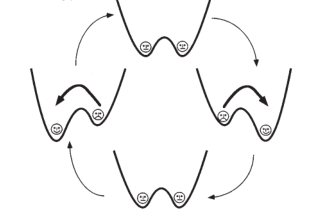
\includegraphics[width=20em]{000.png}
\caption{Illustration of cross-region mixing for pixels in
textural image regions. The value of pixel x is denoted as I(x),
and the dotted lines indicate the weights derived by different filters.
Note that we intentionally disregard noisy pixels between
pixels p and q, so that the characteristics of geodesic filters can be
better illustrated.
}
\label{fig:lable}
\end{figure}\\
\section{Propagation Filtering}
As illustrated in Figure 1, cross-region mixing is a typical problem for existing filters when performing image processing tasks like denoising or smoothing. For example, although bilateral filters measure the photometric distances between pixels for determining the filter weights, their use of explicit spatial filtering kernels would inevitably assign weights to pixels across image regions\cite{Mclaughlin2001Theory}. On the other hand, geodesic filters utilize image context information for filtering by accumulating the value differences from adjacent pixels. However, when adjacent image regions are of different types of context but noise-free, it would not be able to suppress their effects and thus result in cross-region mixing\cite{Ntziachristos2010Going}.\\
\begin{figure}[htbp]
\small
\centering
\includegraphics[width=20em]{001.png}
\caption{Illustration of propagation filtering. (a) the definition of
filtering weight Ws,t, (b) the calculation of Ws,t, and (c) the pattern
for performing 2D filtering with d $=$ 3 pixels.
}
\label{fig:lable}
\end{figure}\\
\section{Conclusion}
As a local filter operator, the propagating filter is designed to preserve the image context information while smoothing the image\cite{Ruaux2013Enteroscopy}. Although the same target is shared to keep the details of the image as a bilateral and guided filter, the propagation filter is based on the photometric relationship observed between the pixels of the image. Without the use of explicit spatial filtering function, the cross region mixing problem in filtering process can be reduced, thus preserving image features better.
{\small
\bibliographystyle{ieee}
\bibliography{1}
}
\end{document}
